% A loop around the puncture in C \ {0}; the hole is drawn as a meteor.
% Source: book/tex/topology/fundamental-group.tex (§ Fundamental groups).
\documentclass[border=2mm]{standalone}
\usepackage{tikz}
\usepackage{amssymb}
\usetikzlibrary{arrows.meta,decorations.markings}
\begin{document}
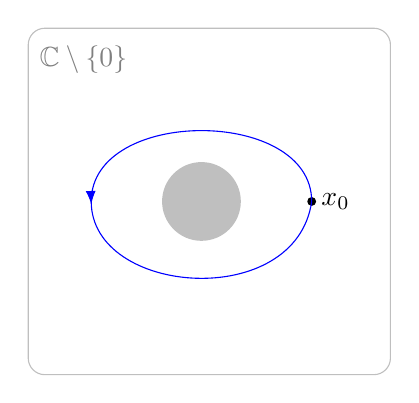
\begin{tikzpicture}[scale=1]
  \draw[rounded corners=6pt, gray!50] (-2.2,-2.2) rectangle (2.4,2.2);
  \node[gray] at (-1.5,1.8) {$\mathbb{C}\setminus\{0\}$};
  \fill[gray!50] (0,0) circle (0.5);
  \fill (1.4,0) circle (1.6pt) node[right] {$x_0$};
  \draw[blue,decoration={markings,mark=at position 0.5 with {\arrow{Latex}}},
    postaction={decorate}]
    (1.4,0) .. controls (1.4,1.2) and (-1.4,1.2) .. (-1.4,0)
            .. controls (-1.4,-1.2) and (1.2,-1.4) .. (1.4,0);
\end{tikzpicture}
\end{document}
